\chapter{Plano de Teste}
\label{Plano de Teste}

O plano de testes:

Para deixar o bot mais preciso e confiável, faremos alguns testes com ele.:
Faremos um teste para conferir se o bot está liderando/dominando a conversa, para que o usuário não desvie do assunto principal. O ideal é que o bot tenha uma conversa fluida com o usuário. 
Testaremos também o vocabulário (Teste de Domínio). É preciso que o bot tenha um vocabulário extenso, incluindo gírias , dialetos e possíveis formas de falar a mesma frase. 

Faremos testes com grupos de pessoas internas e externas utilizando o plano de testes descrito acima. 
\begin{itemize}

\item \textbf {Primeiro:} Teste manual, entre nós mesmos. 

\item \textbf {Segundo:} será feito entre os grupos da sala. Será testado a eficiência do bot quanto ao domínio e a liderança na conversa. 

\item \textbf {Terceiro teste:} Este será feito com pessoas externas. Nosso critério de escolha é dar maior atenção para o nosso público alvo. Faremos teste com pessoas da família que tem menos conhecimento sobre o mundo virtual/tecnologia e com pessoas da família que tenha um pouco mais de conhecimento. Este teste será feito entorno de 10 à 15 pessoas.
\end{itemize}
Como o bot é aberto para todos, faremos também com pessoas que tem mais conhecimento na área, podendo ser pessoas de outros períodos ou até mesmo com mais pessoas da nossa sala. Este teste será feito entre 5 à 10 pessoas.

Como vão saber quando o bot não soube responder? 

Acompanharemos pela ferramenta toda a conversação de testes. No Chatfuel, é possível ver mensagens enviadas pelo usuário que ainda não foram automatizadas. As mensagens que tem ligação direta com o assunto, serão automatizadas após e durante a fase de testes. 

Onde nosso pode ser encontrado projeto? 

A versão final do projeto será disponibilizada no Facebook. Escolhemos o Facebook por  ser uma  plataforma mais acessível, visto  que o projeto é voltado para um público com pouco conhecimento do mundo virtual. As pessoas poderão se comunicar com o bot pelo Facebook Messenger.

\section{Plataforma Utilizada}
\label{Plataforma Utilizada}
    Utilizamos a plataforma "Facebook" para hospedar nosso bot, ela oferece diversidade de respostas e a possibilidade de implementação através da indução ao erro, o serviço do mesmo é gratuito.\\
\begin{figure}[h]
\centering
\captionsetup[subfigure]{labelformat=empty}
\caption{``Bot Anna''}
\begin{subfigure}{.5\textwidth}
\centering
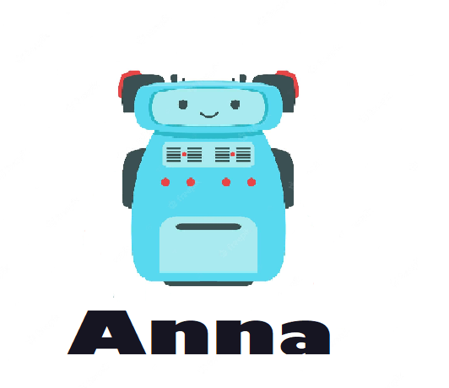
\includegraphics[width=8cm,height=6cm]{Partes/Imagens/Anna.png}
\caption{Bot criado pelo grupo (2022).}
\end{subfigure}%
\end{figure}

\section{Gráficos de confiabilidade do bot}
\label{Gráficos de confiabilidade do bot}
\begin{figure}[h]
\flushleft
\captionsetup[subfigure]{labelformat=empty}
\caption{``Acerto do perguntas de um Iniciante''}
\begin{subfigure}{.5\textwidth}
\centering
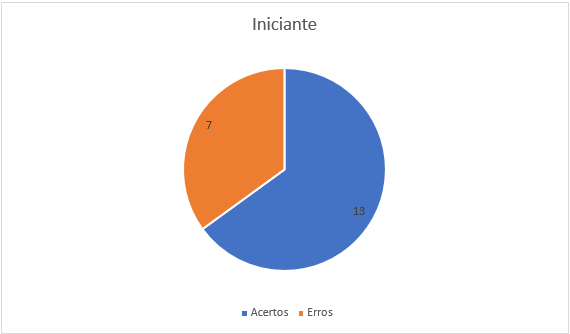
\includegraphics[width=16cm,height=8cm]{Partes/Imagens/Iniciante.png}
\end{subfigure}%
\end{figure}

\begin{figure}[h]
\flushleft
\captionsetup[subfigure]{labelformat=empty}
\caption{``Acerto do perguntas de um Avançado''}
\begin{subfigure}{.5\textwidth}
\centering
\includegraphics[width=16cm,height=8cm]{Partes/Imagens/Avançado.png}
\end{subfigure}%
\end{figure}